\section{Background}
\label{sec:background}

Machine learning is the field of artificial intelligence responsible for 
learning from data without being explicitly programmed to do so. In this way, 
the results provided by the algorithm do not depend on how data is processed, 
but rather on data itself. Obviously, it is not possible to define a single 
algorithm for all possible learning problems.

There are mainly two methods to train an algorithm on a dataset: 
\textit{supervised} and \textit{unsupervised} learning. In supervised learning, 
we provide a label to specify which value is associated to each entry in the 
dataset. Consequently, we are able to train the algorithm based on examples. 
In unsupervised learning, there is no label for each entry. Thus, to 
determinate if two examples are referring to the same result, we need a 
\textit{similarity measure} (e.g. if we represent data using vector, one 
possible measure of similarity is cross product).

\textit{Pattern Matching} is the branch of machine learning responsible for 
detecting pattern and regularities in data. Typically, it is implemented 
through supervised learning: the dataset is composed by examples with an 
associated label. In this way, the algorithm learns which are the features of a 
specific pattern.
One of the most used method in machine learning for image classification is 
\textit{Deep learning}: this technique uses an Artificial Neural Network 
(\textit{ANN}) - which is a Neural Network (\textit{NN}) composed by more than 
one hidden layer, as shown in Figure~\ref{fig:nn} - in order to classify an 
image, based on similarity measures (unsupervised) or training examples 
(supervised). Typically, NNs use a \textit{backpropagation} algorithm, composed 
of two phases: \textit{feed forward} and \textit{backward propagation}. Firstly, 
the image is decomposed in a vector-like representation. Secondly, during feed 
forward phase, the vector is fed as input to the NN and it is computed. Finally, 
during back propagation, the result of feed forward phase is compared to the 
real label; in case of mismatch, the wrong parts are backpropagated into the NN 
in order to compensate the wrong implementation. This process is repeated for 
each entry in the dataset.

\begin{figure}[htpb]
\centering
    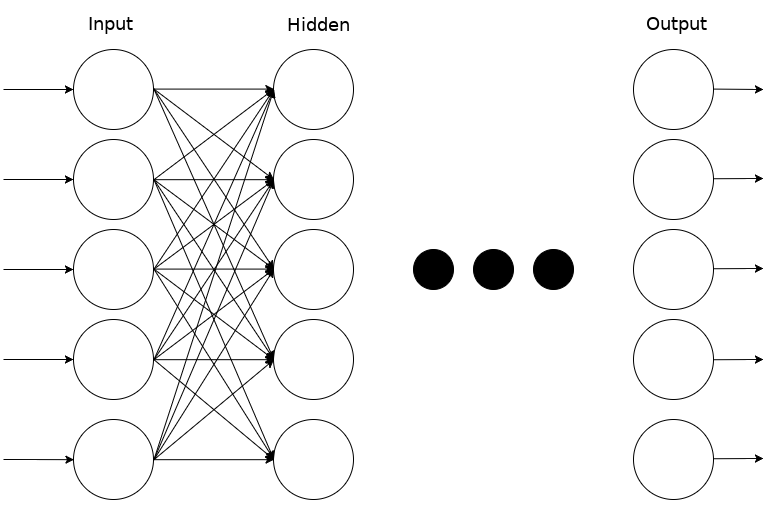
\includegraphics[scale=0.28]{../img/nn}
    \caption{Architecture of a Neural Network}
    \label{fig:nn}
\end{figure}

Deep Neural Networks (DNNs) can use the same principles of NNs, which implement 
backpropagation, but decompose data on many levels (thus "deep" network).

This method is based on the assumption that data can be \textit{abstracted} or 
\textit{composed} in many levels, simplifying the task of comparing pieces of 
data.
Usually, for \textit{computer vision} tasks (e.g. \cite{Handwritten}) 
\textit{Convolutional Neural Networks} (CNNs) are used \cite{CNN}.
However, this algorithms do not have perfect performances: in some cases, the 
labels assigned to an image may be wrong. As a tradeoff between reliability and 
feasibility, classifiers usually assign a \textit{probability} to a certain 
label. 
In this way, who uses the algorithm can decide a threshold to keep/discard 
classifications. 